%\documentclass[12pt,a4paper]{report}
%\usepackage[utf8]{inputenc}
%\usepackage{amsmath}
%\usepackage{amsfonts}
%\usepackage{amssymb}
%\usepackage[margin=2.5cm]{geometry}
%\usepackage{graphicx}
%\usepackage{caption}
%\usepackage{subcaption}
%\usepackage[nottoc,numbib]{tocbibind}
%\linespread{1.3}
%\DeclareMathOperator\sgn{sgn}
%\begin{document}
	\chapter{Three Dimensional Topological Dirac Semimetals}
	\label{weyl}
		The recent influx of study into the two dimensional material graphene has highlighted the field of gapless semiconductors. In graphene the conduction and valence bands meet at a point known as a Dirac point \cite{b1} and massless charge carriers follow a linear energy-momentum relation \cite{b11}. Due to the linear dispersion relation, high Fermi velocity ($v_{f}\approx c/300$) and massless charge carriers, graphene quasiparticles can be modelled by the relativistic Dirac equation \cite{b12}.

		The results obtained in graphene are equally applicable to a broad class of materials generally named topological insulators \cite{b41, b71}.  In \cite{b41} it was shown that on the interface between the two insulating semiconductors CdTe and HgTe(Se) an inverted band structure may arise. The inverted band structure creates a metallic conducting layer associated with the Dirac gapless spectrum. The single Dirac point is protected by a time reversal symmetry and the conductivity in the Dirac point at zero temperature tends to infinity.

		Three dimensional materials such as Ag$_{2}$Se and Ag$_{2}$Te have been shown to act as small gap semiconductors \cite{b23, b24} and Ag$_{2}$Te can experience a phase transition from narrow-gap semiconductor to gapless semiconductor with a linear spectrum \cite{b25}. Other materials such as grey tin \cite{b26} and mercury telluride \cite{b27} have been shown to possess zero-gap properties with a parabolic dispersion relation. In the case of mercury telluride the size of the energy gap can be adjusted by replacing atoms of mercury with the lighter element cadmium. With a specific concentration of cadmium the dispersion relation becomes gapless and linear \cite{b28}.
		
		Recently, Na$_{3}$Bi has been shown to possess a three dimensional linear dispersion relation \cite{b29}. The crystal structure of Na$_{3}$Bi forms a hexagonal Brillouin zone in the $k_{x}-k_{y}$ plane similar to the two dimensional material graphene. This forms three dimensional Dirac cones close to the center of the Brillouin zone.
		
		The three dimensional Dirac cones have also been shown in the material Cd$_{3}$As$_{2}$ \cite{b34, b35, b36}. This material possesses a non-symmetrical Dirac cone \cite{b34} in the $k_{y}-k_{z}$ direction and a Fermi velocity 1.5 times greater than that of graphene \cite{b35}. These qualities make Cd$_{3}$As$_{2}$ a good candidate for the exploration of Weyl semimetals and three dimensional Dirac cones.

In order to simply model three dimensional materials with a linear spectrum, a three dimensional Weyl Hamiltonian \cite{b50, b51} can be used:
		\begin{equation}
			\hat{H}=v_{f}\hat{p}\cdot\vec{\sigma}+IV(x)
			\label{weyl-ham}
		\end{equation}
		where $v_{f}$ is the Fermi velocity, $\hat{p}$ is the three dimensional momentum operator, $I$ is the identity matrix, $V\left( x\right)$ is an external potential and $\vec{\sigma}$ are the Pauli spin matrices. This Hamiltonian is a two by two matrix similar to that of the graphene Hamiltonian. The exception here is that for Weyl fermions momentum is not limited to the $x$ and $y$ directions. Due to the similarities with the graphene Hamiltonian it is reasonable to apply the same theoretical methods to Weyl fermions in the hope to provide graphene like properties in a three dimensional material.
		\section{Energy Spectrum}
			The energy spectrum can be obtained from the characteristic equation $\det\left(\hat{H}-E\right)=0$. Expressing the Hamiltonian from Equation (\ref{weyl-ham}) into matrix form and a replacing the potential $V\left( x\right)$ with a constant potential $V$, this equation becomes:
			\begin{align}
				\det
				\left[\begin{array}{ccc}
				V-E+v_{f}\hat{p}_{z}&v_{f}\left(\hat{p}_{x}-i\hat{p}_{y}\right)\\
				v_{f}\left(\hat{p}_{x}+i\hat{p}_{y}\right)&V-E-v_{f}\hat{p}_{z}
				\end{array}\right]
				=0
			\end{align}
			Solving this equation produces a three dimensional graphene like linear dispersion relation:
			\begin{align}
				E&=V\pm \hbar v_{f}\sqrt{k_{x}^{2}+k_{y}^{2}+k_{z}^{2}}
				\\
				&=V\pm \hbar v_{f}k
				\label{weyl-e-k}
			\end{align}
			At this stage the removal of the $z$ direction will perfectly reproduce the graphene dispersion relation \cite{b5}.
		\begin{figure}[h]
			\centerline{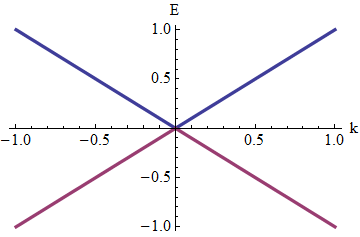
\includegraphics[scale=0.7]{images/weyl-ek}}
			\caption{A plot of energy against momentum from Equation (\ref{weyl-e-k}) with arbitary units. This plot shows the linear dispersion relation of a three dimensional Weyl spinor.}
			\label{}
		\end{figure}
%%%%%
%%%%%
%%%%%
%%%%%
%%%%%
		\section{Wave-functions}
		\label{Weyl - Wave-functions}
			With the energy spectrum of the graphene like Hamiltonian, suitable wave-functions can be selected. These wave-functions can then be used to describe charge carriers in a Weyl semimetal. The time independent Dirac equation in matrix form with the Hamiltonian in Equation (\ref{weyl-ham}) and a constsnt potential can be written as:
			\begin{align}
				\left[\begin{array}{ccc}
				V-E+v_{f}\hat{p}_{z}&v_{f}\left(\hat{p}_{x}-i\hat{p}_{y}\right)\\
				v_{f}\left(\hat{p}_{x}+i\hat{p}_{y}\right)&V-E-v_{f}\hat{p}_{z}
				\end{array}\right]
				\left[\begin{array}{ccc}
				\psi_a\\
				\psi_b
				\end{array}\right]
				=0
			\end{align}
			This equation can then be split into a set of simultaneous equations.
			\begin{equation}
				\left(V-E+v_{f}\hat{p}_{z}\right)\psi_{a}+v_{f}\left(\hat{p}_{x}-i\hat{p}_{y}\right)\psi_{b}=0
				\label{eq1}
			\end{equation}
			\begin{equation}
				v_{f}\left(\hat{p}_{x}+i\hat{p}_{y}\right)\psi_{a}+\left(V-E-v_{f}\hat{p}_{z}\right)\psi_{b}=0
				\label{eq2}
			\end{equation}
			From Equation (\ref{eq2}) the wave-function component $\psi_{b}$ can be shown as an expression of $\psi_{a}$:
			\begin{equation}
				\psi_{b}= -\frac{v_{f}\left(\hat{p}_{x}+i\hat{p}_{y}\right)}{V-E-v_{f}\hat{p}_{z}}\psi_{a}
				\label{weyl-psi-b}
			\end{equation}
			Substituting the value of $\psi_{b}$ into Equation (\ref{eq1}) makes $\psi_{a}$ the only unknown. Using the definition of the momentum operator, Equation (\ref{eq1}) becomes:
			\begin{equation}
				\left(\left(E-V\right)^{2}-\hbar^{2}v_{f}^{2}\left(\frac{\partial^{2}}{\partial x^{2}}+\frac{\partial^{2}}{\partial y^{2}}+\frac{\partial^{2}}{\partial z^{2}}\right)\right)\psi_{a}=0
				\label{eq3}
			\end{equation}
			Requiring that the wave-function be separable and a plane wave in the $y$ and $z$ directions; $\psi_{a}$ is required to be in the form of $f(x)e^{ik_{y}y}e^{ik_{z}z}$. Using these requirements for $\psi_{a}$, Equation (\ref{eq3}) becomes:
			\begin{equation}
				\left(\frac{\left(E-V\right)^{2}}{\hbar^{2}v_{f}^{2}}-k_{y}^{2}-k_{z}^{2}\right)f(x)+f''(x)=0
			\end{equation}
			With the solution:
			\begin{equation}
				f(x)=e^{iqx}\hspace{1 cm}q=\sqrt{\frac{\left(E-V\right)^{2}}{\hbar^{2}v_{f}^{2}}-k_{y}^{2}-k_{z}^{2}}
			\end{equation}
			Therefore the full expression for $\psi_{a}$ is:
			\begin{equation}
				\psi_{a}=e^{iqx+ik_{y}y+ik_{z}z}
			\end{equation}
			Using this definition of $\psi_{a}$ (with appendix Section \ref{Appendix - pz}) and Equation (\ref{weyl-psi-b}), the wave-function component $\psi_{b}$ can be evaluated to:
			\begin{equation}
				\psi_{b}= \frac{\hbar v_{f}\left(q+ik_{y}\right)}{E-V+\hbar v_{f}k_{z}}e^{iqx+ik_{y}y+ik_{z}z}
				\label{weyl-psib-long}
			\end{equation}
			Then by relating the energy momentum relation to spherical coordinate theory the directional momentum can be expressed in terms of incident angles.
			\begin{equation}
				q=\frac{|E-V|}{\hbar v_{f}}\sin(\phi)\cos(\theta)
				\hspace{0.8 cm}
				k_{y}=\frac{|E-V|}{\hbar v_{f}}\sin(\phi)\sin(\theta)
				\hspace{0.8 cm}
				k_{z}=\frac{|E-V|}{\hbar v_{f}}\cos(\phi)
			\end{equation}
			These definitions of momentum can be used to rewrite Equation (\ref{weyl-psib-long}) as:
			\begin{align}
				\psi_{b}&=\frac{|E-V|\sin(\phi)}{E-V+|E-V|\cos(\phi)} e^{iqx+i\theta+ik_{y}y+ik_{z}z}
				\\
				&=\alpha  e^{iqx+i\theta+ik_{y}y+ik_{z}z}
			\end{align}
			Where $\alpha$ is defined as:
			\begin{equation}
				\alpha=\frac{|E-V|\sin(\phi)}{E-V+|E-V|\cos(\phi)}
			\end{equation}
			The full wave-function is then:
			\begin{align}
				\psi=
				\left[\begin{array}{ccc}
					\psi_a\\	
					\psi_b
				\end{array}\right]
				=
				\left[\begin{array}{ccc}
					e^{iqx+ik_{y}y+ik_{z}z}\\	
					\alpha  e^{iqx+i\theta+ik_{y}y+ik_{z}z}
				\end{array}\right]
			\end{align}
			In this form these wave-functions resemble the graphene wave-functions and the theory used for graphene can be directly applied to Weyl fermions.
%%%%%
%%%%%
%%%%%
%%%%%
%%%%%
		\section{The Potential Step}
		\label{weyl - The Step Potential}
			In the same way as the graphene potential barrier, the potential step for a three dimensional gapless semiconductor will require special care when calculating the scattering properties. As the wave-functions have been derived to appear similar to those of graphene, a potential step or barrier which is only present in one dimension will produce identical results to graphene with the exception that the values for $\alpha_{a,b}$ and momentum will maintain their three dimensional nature. This means that the transmission probability through the potential step must be calculated by:
			\begin{equation}
				T=|t|^{2}\frac{\alpha_{b}\cos(\theta_{b})}{\alpha_{a}\cos(\theta_{a})}
			\end{equation}
			instead of the usual $T=|t|^{2}$. The phase of the wave-functions must also be considered within the step; any region of hole transport will require a phase shift of $\theta_{h}=\pi-\theta_{e}$ or $\phi_{h}=-\phi_{e}$ where the subscript $h$ and $e$ represent holes and electrons respectively. With these conditions the transfer matrix method can be used to obtain the transmission probability through the potential step. This method is identical to the graphene case and therefore the result derived in Section \ref{Potential Step - Transfer and Scattering Matrices}:
		\begin{equation}
			T=\frac{4\alpha_{a}\alpha_{b}\cos(\theta_{a})\cos(\theta_{b})}{\alpha_{a}^{2}+\alpha_{b}^{2}+2\alpha_{a}\alpha_{b}\cos(\theta_{a}+\theta_{b})}
			\label{weyl - stept}
		\end{equation}
		can be used with the three dimensional definitions of $\alpha_{a,b}$ and momentum. This result can be reduced to the two dimensional cases by setting the corresponding angle to incidence. To remove the $z$ direction $\phi_{a}$ can be set to $\pi/2$ producing:
		\begin{equation}
			T=\frac{4s_{a}s_{b}\cos(\theta_{a})\cos(\theta_{b})}{s_{a}^{2}+s_{b}^{2}+2s_{a}s_{b}\cos(\theta_{a}+\theta_{b})}
			\label{}
		\end{equation}

		Where $s_{a,b}=\sgn(E-V_{a,b})$. The terms $\sgn(E-V_{a,b})^{2}$ have not been cancelled to allow for the special case where $E=V_{a,b}$. The $y$ direction can then be removed by requiring that $\theta_{a}=0$ which will reduce the transmission probability to:
		\begin{equation}
			T=\frac{4\alpha_{a}\alpha_{b}}{\alpha_{a}^{2}+\alpha_{b}^{2}+2\alpha_{a}\alpha_{b}}
			\label{}
		\end{equation}

		\begin{figure}[h]
			 \begin{subfigure}[h]{0.5\textwidth}
				\centerline{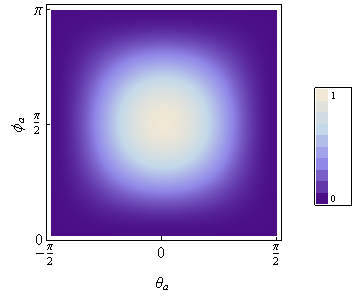
\includegraphics[scale=0.5]{images/weyl-step-phi-theta}}
				\caption{}
			\end{subfigure}
			\hspace{0.5cm}
			\begin{subfigure}[h]{0.5\textwidth}
				\centerline{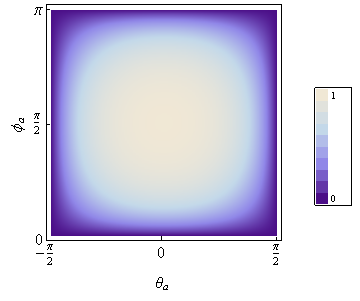
\includegraphics[scale=0.5]{images/weyl-step-phi-theta-2}}
				\caption{}
			\end{subfigure}
			\caption{Density plots for transmission probability against incident angles $\theta_{a}$ and $\phi_{a}$ from Equation (\ref{weyl - stept}) for a potential step with the characteristics $V_{a}=0.1$ eV, $V_{b}=0$ eV. In (a) the angular dependence is shown at energies within the potential step for $E=0.05$ eV. (b) Shows the transmission probability against incident angles $\theta_{a}$ and $\phi_{a}$ at energies outside of the potential step, here $E=-0.05$ eV. }
			\label{weyl-step-1}
		\end{figure}

		\begin{figure}[h]
			 \begin{subfigure}[h]{0.5\textwidth}
				\centerline{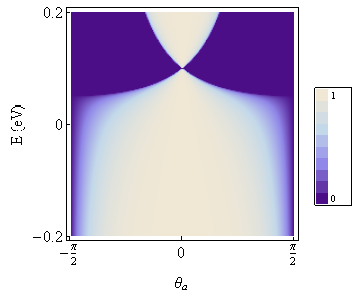
\includegraphics[scale=0.5]{images/weyl-step-theta}}
				\caption{}
			\end{subfigure}
			\hspace{0.5cm}
			\begin{subfigure}[h]{0.5\textwidth}
				\centerline{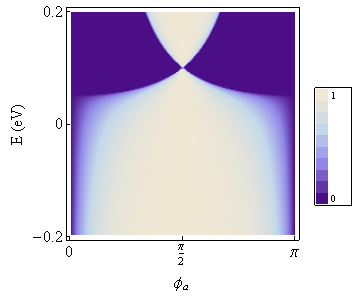
\includegraphics[scale=0.5]{images/weyl-step-phi}}
				\caption{}
			\end{subfigure}
			\caption{Density plots for transmission probability against energy and incident angles $\theta_{a}$ and $\phi_{a}$ from Equation (\ref{weyl - stept}) for a potential step with the characteristics $V_{a}=0.1$ eV, $V_{b}=0$ eV. In (a) the transmission probability is plotted against energy and $\theta_{a}$ with $\phi_{a}=\pi/2$. (b) The transmission probability against energy and $\phi_{a}$ with $\theta_{a}=0$. }
			\label{weyl-step-2}
		\end{figure}

		The angular symmetry of the potential step can be seen in the density plot in Figure \ref{weyl-step-1}. At all energies for the potential step, the $\theta_{a}$ and $\phi_{a}$ dependencies are equivalent, with the region of perfect transmission increasing away from the step.
%%%%%
%%%%%
%%%%%
%%%%%
%%%%%
		\section{The Potential Barrier}
		\label{weyl - Scattering Properties}
		The wave-functions previously derived in Section \ref{Weyl - Wave-functions} can then be used in the scattering problem described in Figure \ref{weyl-symmetrical-flat}. Here regional subscripts will be added to groups of constants in each region. Continuity of the wave-functions require that at the barrier interface the wave-function to the left must equal the wave-function to the right. As this barrier interface is located at $x=0$, the requirement $\psi_{a}=\psi_{b}$ reduces the wave-functions to:
		\begin{figure}[h]
			\centerline{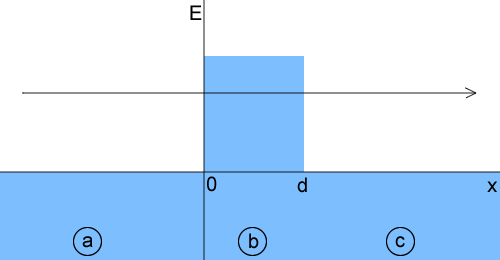
\includegraphics[scale=0.7]{images/weyl-symmetrical-flat}}
			\caption{The potential barrier problem. A potential barrier is placed in the $x$ direction with a height $V_{b}$ and a width $d$. The shaded region shows where hole transport is present. The three independent regions have been labelled as $a,b$ and $c$.}
			\label{weyl-symmetrical-flat}
		\end{figure}

		\begin{align}
			\left[\begin{array}{ccc}
				1&1\\
				\alpha_{a}e^{i\theta_{a}}&-\alpha_{a}e^{-i\theta_{a}}
			\end{array}\right]
			\left[\begin{array}{ccc}
				a_{1}\\
				a_{2}
			\end{array}\right]
			&=
			\left[\begin{array}{ccc}
				1&1\\
				\alpha_{b}e^{i\theta_{b}}&-\alpha_{b}e^{-i\theta_{b}}
			\end{array}\right]
			\left[\begin{array}{ccc}
				a_{3}\\
				a_{4}
			\end{array}\right]
		\end{align}
		Where again, the notation $m_{1}$ and $m_{2}$ represents the wave-functions to the left and right of the barrier interface respectively.
		\begin{align}
			m_{1}\left[\begin{array}{ccc}
				a_{1}\\
				a_{2}
			\end{array}\right]
			&=
			m_{2}\left[\begin{array}{ccc}
				a_{3}\\
				a_{4}
			\end{array}\right]
		\end{align}
		At the second boundary located at $x=d$ the wave-function on the left of the interface must equal the wave-function on the right, which will be written as:
		\begin{align}
			\left[\begin{array}{ccc}
				e^{iq_{b}d}&e^{-iq_{b}d}\\
				\alpha_{b}e^{iq_{b}d+i\theta_{b}}&-\alpha_{b}e^{-iq_{b}d-i\theta_{b}}
			\end{array}\right]
			\left[\begin{array}{ccc}
				a_{3}\\
				a_{4}
			\end{array}\right]
			&=
			\left[\begin{array}{ccc}
				e^{iq_{c}d}&e^{-iq_{c}d}\\
				\alpha_{c}e^{iq_{c}d+i\theta_{c}}&-\alpha_{c}e^{-iq_{c}d-i\theta_{c}}
			\end{array}\right]
			\left[\begin{array}{ccc}
				a_{5}\\
				a_{6}
			\end{array}\right]
		\end{align}
		With $m_{3}$ and $m_{4}$ defined so that:
		\begin{align}
			m_{3}\left[\begin{array}{ccc}
				a_{3}\\
				a_{4}
			\end{array}\right]
			&=
			m_{4}\left[\begin{array}{ccc}
				a_{5}\\
				a_{6}
			\end{array}\right]
		\end{align}
		Using these definitions the constants $a_{3}$ and $a_{4}$ can be eliminated and the transfer matrix $M$ becomes:
		\begin{align}
			\left[\begin{array}{ccc}
				a_{5}\\
				a_{6}
			\end{array}\right]=M
			\left[\begin{array}{ccc}
				a_{1}\\
				a_{2}
			\end{array}\right]\hspace{1cm}
			M=m_{4}^{-1}m_{3}m_{2}^{-1}m_{1}
		\end{align}
		Evaluating the transfer matrix allows the transmission coefficient and the transmission probability to be obtained. From transfer matrix theory $t=1/M_{2,2}$ and $T=|t|^{2}$ resulting in:
		\begin{equation}
			t=\frac{2\alpha_{a}\alpha_{b}e^{-iq_{a}d}\cos(\theta_{a})\cos(\theta_{b})}{2\alpha_{a}\alpha_{b}\left(\cos(q_{b}d)\cos(\theta_{a})\cos(\theta_{b})+i\sin(q_{b}d)\sin(\theta_{a})\sin(\theta_{b})\right)-i\sin(q_{b}d)\left(\alpha_{a}^{2}+\alpha_{b}^{2}\right)}
		\end{equation}
		\begin{equation}
			T=\frac{4\alpha_{a}^{2}\alpha_{b}^{2}\cos^{2}(\theta_{a})\cos^{2}(\theta_{b})}{4\alpha_{a}^{2}\alpha_{b}^{2}\cos^{2}(q_{b}d)\cos^{2}(\theta_{a})\cos^{2}(\theta_{b})+\sin^{2}(q_{b}d)\left(2\alpha_{a}\alpha_{b}\sin(\theta_{a})\sin(\theta_{b})-\alpha_{a}^{2}-\alpha_{b}^{2}\right)^{2}}
		\label{weyl-combo-t}
		\end{equation}
		This equation can then be reduced to produce the transmission probability for two dimensional systems. To remove $k_{z}$ the angle $\phi_{a}$ can be set to $\pi /2$ resulting in:
		\begin{equation}
			T=\frac{4s_{a}^{2}s_{b}^{2}\cos^{2}(\theta_{a})\cos^{2}(\theta_{b})}{4s_{a}^{2}s_{b}^{2}\cos^{2}(q_{b}d)\cos^{2}(\theta_{a})\cos^{2}(\theta_{b})+\sin^{2}(q_{b}d)\left(2s_{a}s_{b}\sin(\theta_{a})\sin(\theta_{b})-s_{a}^{2}-s_{b}^{2}\right)^{2}}
		\end{equation}
		where $s_{a,b}=\sgn(E-V_{a,b})$. This result recreates the graphene result in \cite{b1}, however, the $s_{a,b}^{2}$ terms have not been removed to allow for special case results when $E=V_{a,b}$. Similarly the $y$ dimension can be removed from Equation (\ref{weyl-combo-t}) by setting the angle $\theta_{a}=0$. Therefore the result for a two dimensional material in the $x-z$ plane can be reduced to:
		\begin{equation}
			T=\frac{4\alpha_{a}^{2}\alpha_{b}^{2}}{4\alpha_{a}^{2}\alpha_{b}^{2}\cos^{2}(q_{b}d)+\sin^{2}(q_{b}d)\left(\alpha_{a}^{2}+\alpha_{b}^{2}\right)^{2}}
		\end{equation}

		As the wave-functions were expressed in an identical form to the graphene wave-functions it is unsurprising that the result for the transmission probability is identical to the graphene case. However, as the constants involved vary from the graphene case the overall result is expected to differ significantly.
	
		The density plots in Figure \ref{weyl-1} show the transmission probability through a potential barrier. In Figure \ref{weyl-1} (a) the incident energy is within the barrier, here the transmission probability is symmetrical for both incident angles. The plot also shows resonances and high transimssion probability when both angles are near incidence. In Figure \ref{weyl-1} (b) the energy is well below barrier height, the plot remains symmetrical, with the region of perfect transmission increasing away from the barrier.
		\begin{figure}[h]
			 \begin{subfigure}[h]{0.5\textwidth}
				\centerline{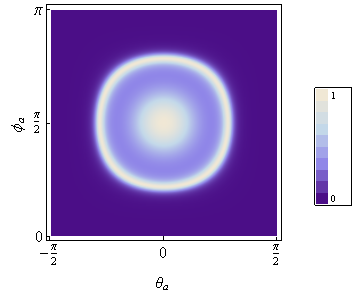
\includegraphics[scale=0.5]{images/weyl-barrier-phi-theta}}
				\caption{$E=0.05$ eV}
			\end{subfigure}
			\hspace{0.5cm}
			\begin{subfigure}[h]{0.5\textwidth}
				\centerline{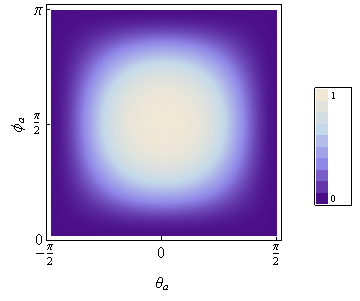
\includegraphics[scale=0.5]{images/weyl-barrier-phi-theta-2}}
				\caption{$E=-0.05$ eV}
			\end{subfigure}
			\caption{Density plots for the transmission probability from Equation (\ref{weyl-combo-t}) against incident angles $\theta_{a}$ and $\phi_{a}$ for a potential barrier with height $V_{b}=0.1$ eV and width $d=100$ nm.}
			\label{weyl-1}
		\end{figure}

		By setting one angle to be normal to the barrier, the dependence of the other angle can be examined in further detail. Angle $\theta_{a}$ has been set to zero in Figure \ref{weyl-3} (a) so that the $\phi_{a}$ dependence can be shown. Extra resonances are added at regular energy intervals with the $\phi_{a}$ dependence centering at barrier height. When $\phi_{a}$ is set to normal incidence the three dimensional barrier is reduced to the two dimensional case shown in graphene.
		\begin{figure}[h]
			 \begin{subfigure}[h]{0.5\textwidth}
				\centerline{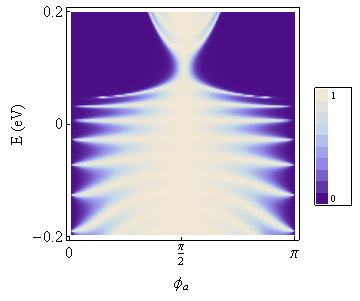
\includegraphics[scale=0.5]{images/weyl-bar-phi}}
				\caption{$\theta_{a}=0$}
			\end{subfigure}
			\hspace{0.5cm}
			\begin{subfigure}[h]{0.5\textwidth}
				\centerline{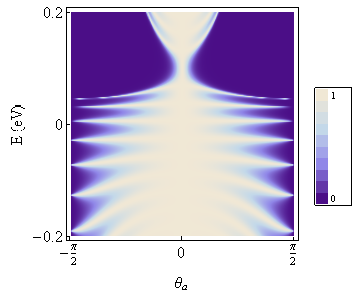
\includegraphics[scale=0.5]{images/weyl-bar-theta}}
				\caption{$\phi_{a}=\pi/2$}
			\end{subfigure}
			\caption{Density plots for the transmission probability from Equation (\ref{weyl-combo-t}) against energy and incident angle with one fixed angle. The potential barrier has a height $V_{b}=0.1$ eV and width $d=100$ nm.}
			\label{weyl-3}
		\end{figure}
%%%%%
%%%%%
%%%%%
%%%%%
%%%%%
		\section{Resonances and Bound States}
		\label{weyl - Resonances and Bound States}
			As the result for the transmission probability is identical to the graphene case, the same resonance condition applies to Weyl fermions. Resonances can occur when the transmission probability is equal to one. From the equation for transmission probability in Equation (\ref{weyl-combo-t}) this condition is satisfied when $q_{b}d=n\pi$. With the three dimensional definition of $q_{b}$ the resonances can be found with:
			\begin{equation}
				E=V_{b}\pm\hbar v_{f}\sqrt{\frac{n^{2}\pi^{2}}{d^{2}}+k_{y}^{2}+k_{z}^{2}}
				\label{weyl-resonances}
			\end{equation}

			The result in Figure \ref{weyl-3} shows an increase of resonances at energies away from barrier height. To find the number of resonances at a specific energy the angular dependence in Equation (\ref{weyl-resonances}) can be removed. With no angular dependence the number of resonances can be found with the equation:
			\begin{equation}
				n=\pm\frac{d\left(E-V_{b}\right)}{\hbar v_{f}\pi}
			\end{equation}

			The three resonances present at $E=0.05$ eV for a barrier with height $0.1$ eV are shown in Figure \ref{weyl-res-1}.
			\begin{figure}[h]
				 \begin{subfigure}[h]{0.5\textwidth}
					\centerline{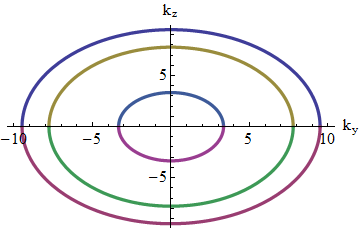
\includegraphics[scale=0.5]{images/weyl-res-1}}
					\caption{}
				\end{subfigure}
				\hspace{0.5cm}
				\begin{subfigure}[h]{0.5\textwidth}
					\centerline{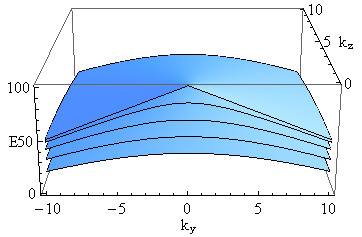
\includegraphics[scale=0.5]{images/weyl-res-2}}
					\caption{}
				\end{subfigure}
				\caption{Fabry-P\'{e}rot resonances from Equation (\ref{weyl-resonances}) inside a potential barrier with height $V_{b}=0.1$ eV and $d=200$ nm. (a) The three resonances present inside the barrier at $E=0.05$ eV. (b) A three dimensional plot of the first four resonances and the result for $n=0$.}
				\label{weyl-res-1}
			\end{figure}

			Graphene potential barriers can create bound states within a single barrier \cite{b3}. The same method can be applied to Weyl fermions to check for the presence of bound states. A bound state only occurs with a system of growth-oscillatory-decay wave-functions. The oscillatory wave-functions used for the potential barrier must therefore be combined with growth or decay wave-functions. Growth-decay wave-functions can be obtained by requiring that $\psi_{a}$ be of the form of exponential growth or decay in the $x$ direction. Separability of the wave-function requires oscillatory wave-functions in the $y$ and $z$ directions. The $\psi_{a}$ component of the wave-function must then be represented as:
			\begin{equation}
				\psi_{a}=e^{q_{d}x+ik_{y}y+ik_{z}z}
			\end{equation}
			The second component of the wave-function can then be found from the definition of $\psi_{b}$ from Equation (\ref{weyl-psi-b}):
			\begin{equation}
				\psi_{b}= -\frac{v_{f}\left(\hat{p}_{x}+i\hat{p}_{y}\right)}{V-E-v_{f}\hat{p}_{z}}e^{q_{d}x+ik_{y}y+ik_{z}z}
			\end{equation}
			Evaluating the momentum operator in all directions produces the $\psi_{b}$ component of the wave-function:
			\begin{equation}
				\psi_{b}= \frac{i\hbar v_{f}\left(q_{d}-k_{y}\right)}{V-E-\hbar v_{f}k_{z}}e^{q_{d}x+ik_{y}y+ik_{z}z}
			\end{equation}
			With the full wave-function, an expression for the unknown $q_{d}$ can be found. By substituting $\psi_{a}$ and $\psi_{b}$ into Equation (\ref{eq1}):
			\begin{equation}
				\left(V-E+v_{f}\hat{p}_{z}\right)e^{q_{d}x+ik_{y}y+ik_{z}z}+v_{f}\left(\hat{p}_{x}-i\hat{p}_{y}\right)\frac{i\hbar v_{f}\left(q_{d}-k_{y}\right)}{V-E-\hbar v_{f}k_{z}}e^{q_{d}x+ik_{y}y+ik_{z}z}=0
			\end{equation}
			Evaluating the operators shows a value of $q_{d}$ which satisfies the Dirac equation for growth-decay wave-functions:
			\begin{equation}
				q_{d}=\sqrt{k_{y}^{2}+k_{z}^{2}-\frac{\left(E-V\right)^{2}}{\hbar^{2}v_{f}^{2}}}
				\hspace{1cm}
				\alpha_{\pm}=\frac{\hbar v_{f}\left(\pm q_{d}+ k_{y}\right)}{E-V_{\pm}+\hbar v_{f}k_{z}}
			\end{equation}
			With these definitions the growth-decay wave-function is of the form:
			\begin{align}
				\psi_{\pm}=
				\left[\begin{array}{ccc}
					\psi_a\\	
					\psi_b
				\end{array}\right]
				=
				\left[\begin{array}{ccc}
					e^{\pm q_{d}x+ik_{y}y+ik_{z}z}\\	
					i\alpha_{\mp} e^{\pm q_{d}x+ik_{y}y+ik_{z}z}
				\end{array}\right]
			\end{align}
			Where the $\pm$ term denotes the exponential growth or decay part of the wave-function. With the definitions of the three dimensional wave-functions, the method for finding graphene bound states in Section \ref{Rectangular Barrier - Bound States} can be applied to the three dimensional case. The system of simultaneous equations at each boundary produces the matrix: 
			\begin{equation}
				\left[\begin{array}{cccc}
					1&-1&-1&0\\
					i\alpha_{-}&-\alpha_{b}&\alpha_{b}^{*}&0\\
					0&e^{iqd}&e^{-iqd}&-e^{-q_{d}d}\\
					0&\alpha_{b} e^{iqd}&-\alpha_{b}^{*} e^{-iqd}&-i\alpha_{+}e^{-q_{d}d}
				\end{array}\right]
				\left[\begin{array}{cccc}
					a_{1}\\
					a_{2}\\
					a_{3}\\
					a_{4}
				\end{array}\right]=
				\left[\begin{array}{cccc}
					0\\
					0\\
					0\\
					0
				\end{array}\right]
			\end{equation}
			Setting the determinant of this matrix to zero produces the equation:
			\begin{equation}
				\tan(q_{b}d)=-\frac{\varepsilon q\left(\alpha_{+}-\alpha_{-}\right)}{-\alpha_{-}\alpha_{+}+\alpha_{b}\alpha_{b}^{*}+\varepsilon k_{y}\left(\alpha_{+}+\alpha_{-}\right)}
				\label{weyl-bound-combo}
			\end{equation}
			where $\varepsilon =\hbar v_{f}/\left(E-V_{b}+\hbar v_{f}k_{z}\right)$. This result can then be used to obtain the energy spectrum for the bound states with respect to $k_{y,z}$. By setting $k_{z}=0$, the bound states in the $y$ direction can be obtained:
			\begin{equation}
				\tan(q_{b}d)=-\frac{q_{d}q}{\frac{E\left(E-V_{b}\right)}{\hbar^{2}v_{f}^{2}}-k_{y}^{2}}
			\end{equation}
			perfectly recreating the result for the two dimensional material graphene as previously derived in \cite{b3}. The $k_{z}$ dependence can then be highlighted by setting $k_{y}=0$:
			\begin{equation}
				\tan(q_{b}d)=-\frac{2q_{d}q}{\frac{\varepsilon_{1}}{\varepsilon}q_{d}^{2}+\frac{\varepsilon}{\varepsilon_{1}}q^{2}}
			\end{equation}
			where $\varepsilon_{1} =\hbar v_{f}/\left(E+\hbar v_{f}k_{z}\right)$.
% In Figure \ref{weyl-bound-states-ky} the bound states have been shown with respect to $k_{y,z}$. It is clear that the appearance of bound states is symmetrical with respect to $k_{y}$ and $k_{z}$.
%		\begin{figure}[h]
%			 \begin{subfigure}[h]{0.5\textwidth}
%				\centerline{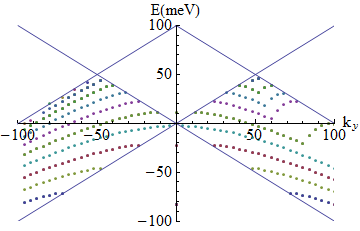
\includegraphics[scale=0.6]{images/weyl-bound-y}}
%				\caption{The $k_{y}$ dependence on the bound states with $k_{z}=0$.}
%			\end{subfigure}
%			\hspace{0.5cm}
%			\begin{subfigure}[h]{0.5\textwidth}
%				\centerline{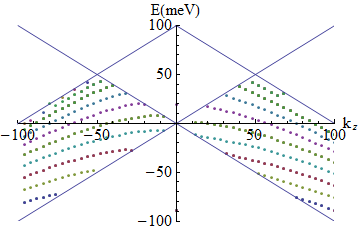
\includegraphics[scale=0.6]{images/weyl-bound-z}}
%				\caption{The $k_{z}$ dependence on the bound states with $k_{y}=0$.}
%			\end{subfigure}
%			\caption{The bound states within a potential barrier from Equation (\ref{weyl-bound-combo}) with a height $0.1$ eV, width $d=200$ nm and $\hbar v_{f}=1$. The boundaries between transport regions have been included in these diagrams to show the valid regions for transport and bound states.}
%			\label{weyl-bound-states-ky}
%		\end{figure}
%%%%%
%%%%%
%%%%%
%%%%%
%%%%%
%		\section{Asymmetrical Barrier}
%		\label{Weyl - Asymmetrical Barrier}
%		The asymmetrical barrier problem described in Chapter \ref{Asymmetrical Barrier} can be applied to the three-dimensional case. Due to the similarity between the wave-functions for the two-dimensional and three dimensional cases the result for transmission obtained previously can be used:
%		\begin{equation}
%			T=\frac{4\alpha_{a}\alpha_{b}^{2}\alpha_{c}cos(\theta_{a})cos(\theta_{c})cos^{2}(\theta_{b})e^{i\theta_{a}+i\theta_{c}}}{r_{3}r_{4}}
%		\end{equation}
%		where:
%		\begin{align}
%r_{3}&=\alpha_{b}\alpha_{c}cos(dq_{b}-\theta_{b})+\alpha_{a}\alpha_{b}e^{i\theta_{a}+i\theta_{c}}cos(dq_{b}+\theta_{b})+i\left(\alpha_{a}\alpha_{c}e^{i\theta_{a}}+\alpha_{b}^{2}e^{i\theta_{c}}\right)sin(dq_{b})
%			\\
%			r_{4}&=\alpha_{a}\alpha_{b}cos(dq_{b}+\theta_{b})+\alpha_{b}\alpha_{c}e^{i\theta_{a}+i\theta_{c}}cos(dq_{b}-\theta_{b})-i\left(\alpha_{b}^{2}e^{i\theta_{a}}+\alpha_{a}\alpha_{c}e^{i\theta_{c}}\right)sin(dq_{b})
%			\label{weyl-asy-t-combo}
%		\end{align}
%		With the definitions of $\alpha, q$ and $\theta$ in Section \ref{Weyl - Wave-functions} the plots in Figure \ref{asy-3d-phi} were obtained to show the $\theta$ and $\phi$ dependencies. As with the two-dimensional case the direction of the charge carriers at electron-hole interfaces must be considered for asymmetrical barriers. To represent this at energies below the barrier the angles of the holes is changed so that $\theta_{h}=\pi-\theta_{e}$ and $\phi_{h}=-\phi_{e}$ where the subscript $e$ and $h$ represents an electron or a hole respectivly.
%		\begin{figure}[h]
%			 \begin{subfigure}[h]{0.5\textwidth}
%				\centerline{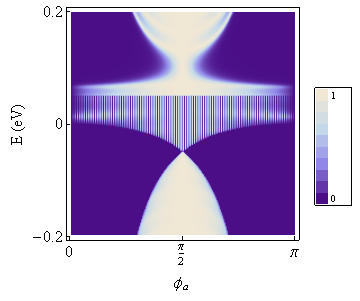
\includegraphics[scale=0.6]{images/weyl-asy-phi}}
%				\caption{The angular dependence on $\phi_{a}$ against energy with $\theta_{a}=0$.}
%			\end{subfigure}
%			\hspace{0.5cm}
%			\begin{subfigure}[h]{0.5\textwidth}
%				\centerline{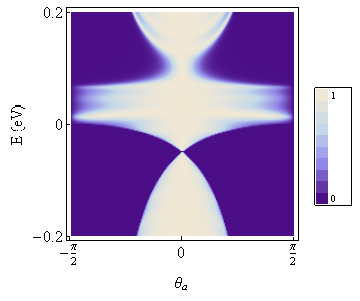
\includegraphics[scale=0.6]{images/weyl-asy-theta}}
%				\caption{The angular dependence on $\theta_{a}$ against energy with $\phi_{a}=\pi/2$.}
%			\end{subfigure}
%			\caption{Density plot of the transmission probability from Equation (\ref{weyl-asy-t-combo}) with energy against incident angle for a three-region system. For both plots $d=100$ nm, $V_{a}=0.05$ eV, $V_{b}=0.1$ eV and $V_{c}=-0.05$ eV.}
%			\label{asy-3d-phi}
%		\end{figure}
%%%%%
%%%%%
%%%%%
%%%%%
%%%%%
		\section{Three Dimensional Superlattice}
		\label{Weyl - Three Dimensional Superlattice}
		In this section a superlattice is constructed from a three dimensional material with a linear energy spectrum. The methods used here are similar to those in Section \ref{Rectangular Barrier - Graphene Superlattice}, where the superlattice structure is compared to an electron in a periodic potential. As the wave-functions for three dimensional graphene are similar to that of two dimensional graphene the result in Equation (\ref{Rectangular Barrier band eq}) can be used.
			\begin{align}
				-\sin(q_{a}d)&\sin(q_{b}d)\left[\frac{\alpha_{a}}{\alpha_{b}}+\frac{\alpha_{b}}{\alpha_{a}}\right]+\sin(q_{a}d)\sin(q_{b}d)\sin(\theta_{a})\sin(\theta_{b})\\
				&+\cos(q_{a}d)\cos(q_{b}d)\cos(\theta_{a})\cos(\theta_{b})-\cos(2kd)\cos(\theta_{a})\cos(\theta_{b})=0
				\label{Rectangular Barrier band eq 3d}
			\end{align}
However, the quantities $\alpha_{a,b}, q_{a,b}$ and $\theta_{a,b}$ must be redefined in three dimensions so that:
			\begin{align}
				q_{a,b}&=\frac{|E-V_{a,}|}{\hbar v_{f}}\sin(\phi_{a,b})\cos(\theta_{a,b})\\
				\alpha_{a,b}&=\sgn(E-V_{a,b})\tan\left(\frac{\phi_{a,b}}{2}\right)\\
				\theta_{a,b}&=\arcsin\left[\frac{\hbar v_{f}k_{y}}{|E-V_{a,b}|\sin(\phi_{a,b})}\right]\\
				\phi_{a,b}&=\arccos\left[\frac{\hbar v_{f}k_{z}}{|E-V_{a,b}|}\right]
			\end{align}
			With these definitions the energy bands of the superlattice can be plotted with respect to the $y$ and $z$ components of momentum shown in Figure \ref{superlattice-bands-3d-ky}.
		\begin{figure}[h]
			 \begin{subfigure}[h]{0.5\textwidth}
				\centerline{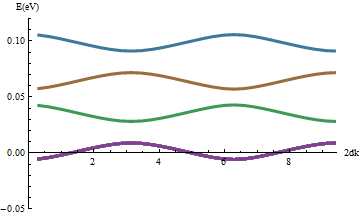
\includegraphics[scale=0.6]{images/energy-bands-0}}
				\caption{The $k$ dependence on the energy bands with $k_{y,z}=0$.}
			\end{subfigure}
			\hspace{0.5cm}
			\begin{subfigure}[h]{0.5\textwidth}
				\centerline{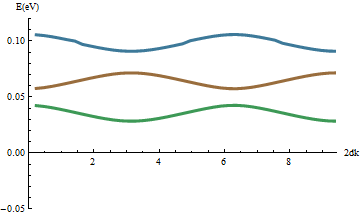
\includegraphics[scale=0.6]{images/energy-bands-ky0}}
				\caption{The $k$ dependence on the energy bands with $k_{y}=0$ and $k_{z}=0.01$.}
			\end{subfigure}
			\caption{The energy bands for an infinite superlattice constructed from a material with a three dimensional linear energy spectrum. To obtain these plots Equation (\ref{Rectangular Barrier band eq 3d}) was used with a barrier height $V_{a}=0.1$ eV and the width $d=50$ nm.}
			\label{superlattice-bands-3d-ky}
		\end{figure}
%%%%%
%%%%%
%%%%%
%%%%%
%%%%%
		\section{Density of States}
		\label{weyl - Density of States}
			The density of states can be caluculated by using the general formula for density of states:
			\begin{equation}
				\rho\left(E\right)=\sum_{k}\delta\left(E-E_{k}\right)
			\end{equation}
			where $\delta\left(x\right)$ is the Dirac delta function. Converting sum notation to integration over all momentum with 2 spin degeneracy:
			\begin{equation}
				\rho\left(E\right)=\frac{L_{x}L_{y}L_{z}}{8\pi^{3}}2\int_{k}\int_{\theta}\int_{\phi}\delta\left(E-E_{k}\right)k^{2}dkd\theta d\phi
			\end{equation}
			With $L_{x,y,z}$ being the size of the system in the respective dimension. Using the linear spectrum of Weyl fermions this can be converted to integration over energy:
			\begin{align}
				E_{k}=\hbar v_{f}k
				\hspace{1cm}
				dE_{k}=\hbar v_{f}dk
				\hspace{1cm}
				k^{2}dk=\frac{E_{k}^{2}}{\hbar^{3}v_{f}^{3}}dE_{k}
			\end{align}
			Finally by using the integration rule $\int f(x)\delta(x) dx=f(0)$ the density of states with 2 valley degeneracy becomes:
			\begin{equation}
				\rho\left(E\right)=\frac{L_{x}L_{y}L_{z}}{\pi\hbar^{3}v_{f}^{3}}E^{2}
			\end{equation}
%%%%%
%%%%%
%%%%%
%%%%%
%%%%%
		\section{IV Characteristics}
		\label{weyl - IV Characteristics}
		In order to find the IV characteristics of a three dimensional, linear spectrum scattering device, the Landauer formalism can be used and is defined as \cite{b6}:
		\begin{equation}
			I=ev_{f}\frac{dn}{dE}T\left(\mu_{1}-\mu_{2}\right)
		\end{equation}
		Using the three dimensional density of states and the transmission probability derived previously, the three dimensional current can be obtained by the same methods as shown in Section \ref{Introduction - Landauer Formalism in Graphene}:
		\begin{equation}
			I_{x}=I_{0}\int^{\infty}_{-\infty}\int^{\pi/2}_{-\pi/2}\int^{\pi}_{0}T\left(E,\theta, \phi\right)\left[f_{L}-f_{R}\right]E^{2}\cos(\theta)\sin(\phi)dEd\theta d\phi
			\label{weyl-i}
		\end{equation}
		With the group of constants $I_{0}=e\frac{2L_{y}L_{z}}{\pi\hbar^{3}v_{f}^{2}}$ and $L_{y,z}$ is the length of the system in the respective direction. In Figure \ref{weyl-vg-1} the current through a Weyl scattering device has been shown with respect to barrier height, source-drain voltage, temperature and Fermi level. The dependence on barrier height is seen in Figure \ref{weyl-vg-1} (a) and Figure \ref{weyl-vg-1} (b). When the source-drain voltage is increased the peak in current which ocurs in Figure \ref{weyl-vg-1} (a) is removed, but the jump in current is still present. 
		\begin{figure}[h]
			\begin{subfigure}[h]{0.5\textwidth}
				\centerline{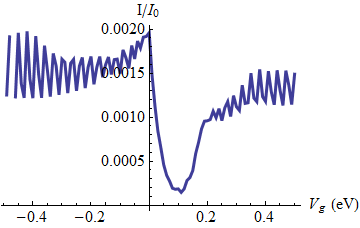
\includegraphics[scale=0.55]{images/weyl-i-1}}
				\caption{$V_{a}=0$ eV and $V_{b}=V_{g}$.}
			\end{subfigure}
			\hspace{0.5cm}
			\begin{subfigure}[h]{0.5\textwidth}
				\centerline{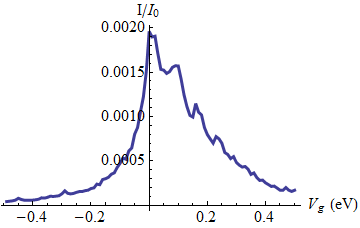
\includegraphics[scale=0.55]{images/weyl-i-2}}
				\caption{$V_{a}=V_{g}$ and  $V_{b}=0$ eV.}
			\end{subfigure}
			\caption{Current against barrier height from Equation (\ref{weyl-i}) with the transmission probability from Equation (\ref{weyl-combo-t}). Here, a potential barrier is constructed from Weyl semimetals with $eV_{sd}=0.1$ eV, $d=100$ nm and $T=298$ K.}
			\label{weyl-vg-1}
		\end{figure}	
		
		 The current with respect to source-drain voltage is also shown in Figure \ref{weyl-g-1} (a), revealing IV characteristics similar to that of a diode. In Figure \ref{weyl-g-1} (b) the temperature dependence is shown to become linear at higher temperatures.
		\begin{figure}[h]
			\begin{subfigure}[h]{0.5\textwidth}
				\centerline{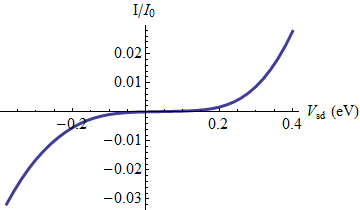
\includegraphics[scale=0.55]{images/weyl-i-vsd}}
				\caption{$T=298$ K}
			\end{subfigure}
			\hspace{0.5cm}
			\begin{subfigure}[h]{0.5\textwidth}
				\centerline{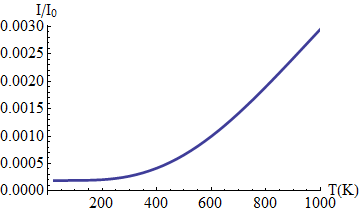
\includegraphics[scale=0.55]{images/weyl-i-t}}
				\caption{$eV_{sd}=0.1$ eV}
			\end{subfigure}
			\caption{Current from Equation (\ref{weyl-i}) with the transmission probability from Equation (\ref{weyl-combo-t}) for Weyl semimetals with $d=100$ nm, $V_{a,c}=0$ eV and $V_{b}=0.1$ eV. (a) Current against source-drain voltage. (b) Current against temperature.}
			\label{weyl-g-1}
		\end{figure}
%%%%%
%%%%%
%%%%%
%%%%%
%%%%%
		\section{Non-symmetrical Dirac Cones}
		\label{weyl - Non-symmetrical Dirac Cone}
		The materials Cd$_{3}$As$_{2}$ \cite{b34, b35} and Na$_{3}$Bi \cite{b29} have recently been shown to possess three dimensional Dirac cones. The experimental results show a Dirac cone with symmetry in the $k_{x}-k_{y}$ plane, however, in the $k_{x}-k_{z}$ plane there was an asymmetry. This asymmetry may cause these materials to behave differently to those with symmetrical Dirac cones. To model this asymmetry a scaling factor $\lambda$ can be introduced to $k_{z}$ so that $k_{z} \rightarrow \lambda k_{z}$. With this change the energy momentum relation changes to:
		\begin{align}
			E&=V\pm \hbar v_{f}\sqrt{k_{x}^{2}+k_{y}^{2}+\lambda^{2} k_{z}^{2}}
			\label{energy-momentum-l}
		\end{align}
		The definition of $k_{z}$ changes to:
		\begin{equation}
			k_{z}=\frac{1}{\lambda}\frac{|E-V|}{\hbar v_{f}}\cos(\phi)
			\label{kz-l}
		\end{equation}
		The effect of this change on the energy momentum relation can be seen in Figure \ref{cone}. Here the symmetrical Dirac cone can be compared to the asymmetrical Dirac cone.
		\begin{figure}[h]
			\begin{subfigure}[h]{0.5\textwidth}
				\centerline{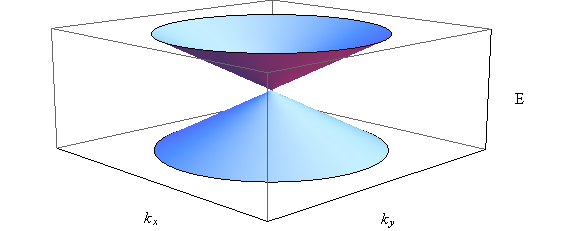
\includegraphics[scale=0.4]{images/cone}}
				\caption{$\lambda^{2}$ = 0.}
			\end{subfigure}
			\hspace{0.5cm}
			\begin{subfigure}[h]{0.5\textwidth}
				\centerline{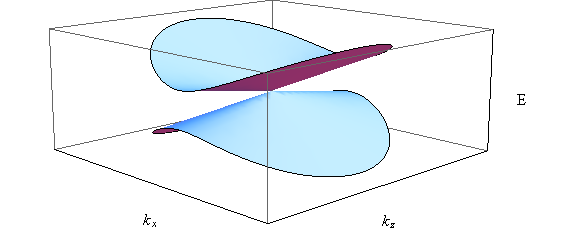
\includegraphics[scale=0.4]{images/cone-z}}
				\caption{$\lambda^{2}$ = 0.1.}
			\end{subfigure}
			\caption{The energy momentum relations for three dimensional Dirac cones with the inclusion of the scaling factor $\lambda$ from Equation (\ref{energy-momentum-l}).}
			\label{cone}
		\end{figure}	

		The change in definition of $k_{z}$ in Equation (\ref{kz-l}) will also affect the scattering properties of any device constructed from these materials. Using the redefined $k_{z}$ and the previously derived result for the potential step in Equation (\ref{weyl - stept}), the rescaled transmission probability has been plotted in Figure \ref{step-l3}. The scaling factor $\lambda$ causes the regions of high transmission to reduce and new regions of no transmission have appeared.
		\begin{figure}[h]
			\begin{subfigure}[h]{0.5\textwidth}
				\centerline{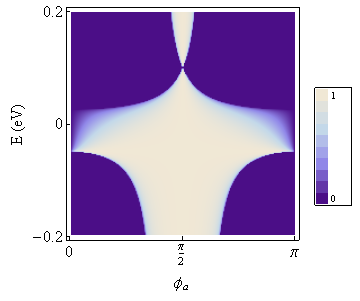
\includegraphics[scale=0.55]{images/step-l3}}
				\caption{$\theta_{a}=0$.}
			\end{subfigure}
			\hspace{0.5cm}
			\begin{subfigure}[h]{0.5\textwidth}
				\centerline{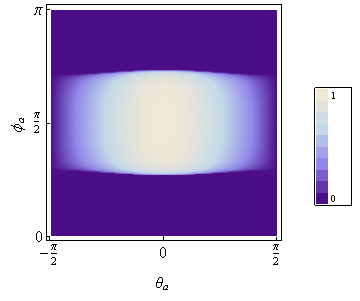
\includegraphics[scale=0.55]{images/phi-theta-step}}
				\caption{$E=-0.1$ eV.}
			\end{subfigure}
			\caption{Density plots for transmission probability against energy and incident angle from Equation (\ref{weyl - stept}) with the modified $k_{z}$ from Equation (\ref{kz-l}). The potential step shown has the characteristics $V_{a}=0.1$ eV, $V_{b}=0$ eV and $\lambda = 1/3$. In (a) the $\theta_{a}$ dependence has been removed to showing energy against $\phi_{a}$. (b) Density plot showing angular dependence at a specific energy $E=-0.1$ eV.}
			\label{step-l3}
		\end{figure}	

		A similar effect is seen when the scaling factor is introduced into the potential barrier case. The plots in Figure \ref{barrier-l3} show the transmission probability for a potential barrier from Equation (\ref{weyl-combo-t}) with $\lambda=1/3$. In addition to the effects witnessed in the potential step case, the resonances that usually occur in the potential barrier become condensed into the reduced regions of transmission. In Figure \ref{barrier-l3} the symmetry of resonances is broken, no longer showing circular resonances but a combination of resonance lines and ovals.
		\begin{figure}[h]
			\begin{subfigure}[h]{0.5\textwidth}
				\centerline{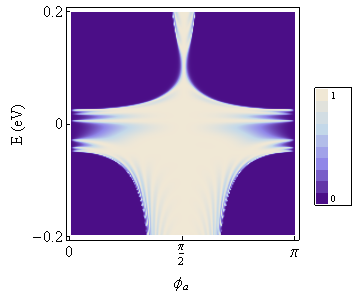
\includegraphics[scale=0.55]{images/barrier-l3}}
				\caption{$\theta_{a}=0$.}
			\end{subfigure}
			\hspace{0.5cm}
			\begin{subfigure}[h]{0.5\textwidth}
				\centerline{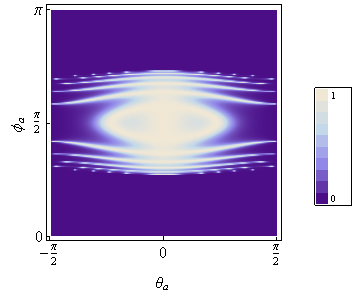
\includegraphics[scale=0.55]{images/phi-theta-barrier}}
				\caption{$E=-0.1$ eV.}
			\end{subfigure}
			\caption{Density plots for transmission probability against energy and incident angle from Equation (\ref{weyl-combo-t}) with the modified $k_{z}$ from Equation (\ref{kz-l}). The potential barrier shown has the characteristics $V_{a}=0$ eV, $V_{b}=0.1$ eV and $\lambda = 1/3$. In (a) the $\theta_{a}$ dependence has been removed to showing energy against $\phi_{a}$. (b) Density plot showing angular dependence at a specific energy $E=-0.1$ eV.}
			\label{barrier-l3}
		\end{figure}	

%%%%%
%%%%%
%%%%%
%%%%%
%%%%%
\section{Conclusion}
\label{Graphene-like properties in three-dimensional gapless semiconductors. - Conclusion}
	Here we have identified the scattering properties and IV characteristics of a three dimensional material with a linear dispersion relation such as Ag$_{2}$Se or Ag$_{2}$Te using a three dimensional Weyl Hamiltonian and vector wave-function.

	The transmission properties through a one dimensional potential barrier show angular symmetry between $\theta_{a}$ and $\phi_{a}$ at all energies. The three dimensional result for transmission probability perfectly reduces to two dimensional results as seen in graphene. Despite a slightly different result when using the $z$ directional momentum, the plots produced for the $x-y$ and $x-z$ show remarkable symmetry. Analysis of the transmission probability through a single potential barrier shows evidence of Fabry-P\'{e}rot resonances and localised bound states in both the $x-y$ and $x-z$ directions. 

	Due to materials Cd$_{3}$As$_{2}$ and Na$_{3}$Bi it is of particular interest to study the transmission properties of a device with an asymmetry between the $x-y$ and $x-z$ directions. The effect of this asymmetry is the introduction of additional regions of no propagation. If any resonances or bound states are present, they are restricted to the reduced transmission regions and therefore the energy between resonances in reduced.

	Using the parabolic density of states and the Landauer formalism the IV characteristics were found for a transistor made from three dimensional materials with a linear dispersion relation. The current shows a non-linear dependence on the source-drain voltage and a linear dependence with respect to high temperatures.
	
	The work here aims to further the understanding of gapless semiconductors and highlight three dimensional materials with graphene like properties. This will allow the pursuit of new materials with relevance to semiconducting devices.
%\end{document}